%!TEX program=pdflatex
%!TEX spellcheck=en_GB
\documentclass{article}
\usepackage[T1]{fontenc}
\usepackage[utf8]{inputenc}
\usepackage{booktabs}
\usepackage{siunitx}
\usepackage{graphicx}
\usepackage{parskip}
\usepackage[eulergreek]{sansmath}
\usepackage{pgfplots}
\pgfplotsset{
	compat=newest,
	tick label style = {font=\sansmath\sffamily\color{white!30!black}},
	every axis label/.append style={font=\color{white!30!black}},
	major grid style={white!30!black},
}
\usepackage{float}
\usepackage{mathtools}
\usepackage{subcaption}
\usepackage[default]{sourcesanspro}
\usepackage[scale=.9]{sourcecodepro}
% \usepackage{fullpage}
\usepackage{enumitem}
\setlist{nosep}
\usepackage{tikz}
\usepackage{siunitx}
\sisetup{detect-all}

\usepackage[backend=biber,texencoding=utf8,bibencoding=utf8,style=ieee,sortlocale=en_US,language=auto]{biblatex}
\makeatletter
\AtEveryBibitem{
    \global\undef\bbx@lasthash}
\makeatother

\usepackage{hyperref}
\hypersetup{ %setup hyperlinks
    colorlinks,
    citecolor=black,
    filecolor=black,
    linkcolor=black,
    urlcolor=black
}

\usepackage[capitalize,noabbrev]{cleveref}
\crefname{appsec}{Appendix}{Appendices}
\captionsetup{width=0.9\textwidth}
\usepackage{standalone}
\usepackage{textcomp}
\usepackage{color}

\setlength{\parskip}{14pt}
\linespread{1.3}
\newlength\figureheight
\newlength\figurewidth

\addbibresource{include/bibliography.bib}

\title{ET4310 -- Supercomputing for Big Data -- Lab 2}
\author{Erwin de Haan (4222814) \and Robin Hes (4236815)}

\begin{document}
\maketitle
\section{Introduction}
In this second assignment of the Supercomputing for Big Data course, a plain-text crawl of the entire internet, the \emph{Common Crawl}, is processed in order to parse every Dutch phone number it contains.
The output is a grouped list of every found number accompanied by the URL(s) at which that particular number was found.
The Amazon \emph{Elastic MapReduce} (EMR) service is employed to enable processing this rather large dataset in a reasonable amount of time.

The aim of the assignment is to optimise the given big data application that is already capable of detecting phone numbers in plain text, in order to attain a certain performance metric.
This metric might be cost, execution time, computational efficiency or anything else that is deemed relevant.

This report will first present a brief analysis of the application, in which possible performance bottlenecks will be identified.
Consequently, this analysis will be used to formulate two independent optimisation strategies along with hypotheses on their effects and any interesting implementation details.
A third section lists the obtained results for the final choice of architecture, after which the report is concluded by a brief summary and future recommendations.

\section{Phone number analysis}
The entire process is of the form of the standard big data pipeline, meaning it can be divided in five consequent stages: Sense/Acquire, Store/Ingest, Retrieve/Filter, Analyse, and Visualise.
Both the sense and store stage have been previously performed, resulting in the Common Crawl as it is provided to the user.
The plain-text part of it consists of a large number of segments that each contain part of the entire set.
The September 2017 (week 39) crawl that will be used in this assignment consists of \num{72000} compressed segments of around \SI{130}{MB} each, making for a total of \SI{8.86}{TB} of compressed data \cite{commoncrawl2017september}.

For the next stage, the retrieval and filtering of data, a script is provided to obtain a list of URLs at which every segment of the dataset may be found.
This list is then used as input to a Pyspark application that takes care of extracting every Dutch phone number it might find, along with the URL it appears on.
The stage is concluded by grouping results by phone number and storing them in a \emph{DataFrame}, which allows convenient access for further processing and analysis.
Note that the retrieval/filtering stage implies a transition from unstructured to structured data, which is the primary interest of this assignment.
The analysis and visualisation stages are not considered here, but as an example one might be interested in the relation between the number's area codes and the sites they are mentioned on, and try to visualise this in a map of some sort.

\subsection{Application profile}

Now, as we try to optimise the Pyspark application, it is important to obtain some insight in the operations it involves.
It can be roughly divided in four consecutive steps:

\begin{enumerate}
	\item Downloading a segment from Amazon's S3 storage and loading it into memory
	\item Decompressing this segment to obtain plain-text data
	\item Extracting phone numbers and URLs (map)
	\item Grouping results and storing them (reduce)
\end{enumerate}

From these steps, potential bottlenecks can already be identified:

\begin{itemize}

	\item The time it takes to a segment is inherently determined by the available network bandwidth from S3 to the EMR cluster.
	\item Decompression is a relatively compute-intensive operation, the performance of which will be limited by the available hardware and used decompression library.
	\item Extracting phone numbers might be compute-intensive as relatively inefficient regular expressions are used in the process.
	\item As these computations are performed in-memory, memory latency and bandwidth might limit performance.
	\item Grouping data involves communication between individual workers, which implies intra-cluster networking overhead.
	\item Storing the results takes time depending on the bandwidth of the storage medium.
\end{itemize}

The first four of this issues are deemed important enough to investigate further, but as the volume of the resulting data (phone numbers and URLs) is expected to be fairly manageable (small), the performance impact of both grouping and storing data should be marginal and is therefore not considered further.

\section{Optimisation}

The bottlenecks identified in the previous section can be simply ascribed to networking, memory and compute performance.
There are several aspects of the process that can be improved to attain higher application performance:

\begin{itemize}
	\item The hardware the application runs on
	\item The way Spark is configured to run the application
	\item The application itself
\end{itemize}

Now, upgrading hardware can alleviate all three of the mentioned bottlenecks, whereas configuring Spark is most likely to improve memory and computational performance, and optimising the application itself can lift some of the computational burden.
The rest of this section will give an overview of the choices that were made with respect to these three aspects.

\subsection{Spark}
Configuring Spark for high performance can be a pain, but several guidelines exist.
\Cref{tab:spark-config} lists the parameters as they were used for the \texttt{spark-submit} command.

\begin{table}[H]
	\caption{Spark configuration}
	\label{tab:spark-config}
	\centering

	\begin{tabular}{llp{6cm}}
	\toprule
	Parameter					& Value	& Explanation \\
	\midrule
	\texttt{--deploy-mode} 		& \texttt{cluster}				& The application master should run on a separate node. \\
	\texttt{--num-executors}	& \# vCPUs		  				& Every vCPU should have at most five executor cores, but a single one is fine when multiple are not required. \\
	\texttt{--executor-cores}	& 1								& See above. \\
	\texttt{--executor-memory}	& $\frac{\text{total memory}}{\text{1.1} \times \text{\# vCPUs}}$	& Spark takes \SI{10}{\percent} of memory as overhead and the rest can be shared among all executors. \\
	\texttt{--driver-cores}		& 1								& No more are required as the application requires little coordination. \\
	\texttt{--driver-memory}	& 2G							& See above. \\
	\bottomrule
	\end{tabular}
\end{table}

The number of partitions (application \texttt{-p} parameter) is equal to twice the total number of vCPUs in the cluster.

\subsection{The application}
The original implementation uses a regular expression to match all Dutch phone numbers in the international format.
Regular expressions are notoriously compute-heavy, so it was an easy target for optimisation.
The replacement is a set of tight loops in a purpose built python C-module.
This alone speeds up the application greatly, and also shifts most of the bottleneck to decompression, networking and IO.
Python passes in a temporary file name, to which the downloaded S3 segment was written.
The module will decompress the full segment to memory and parse the segment byte for byte.
It outputs a list of (phone number, URL) tuples back to python to be picked up by Pyspark.

The implementation is not perfect.
Initially the full extent of correct Dutch phone number recognition was implemented.
This includes special numbers, domestic formatted numbers (checked for correct area codes) and international formatted numbers.
This resulted in huge result sets with many false-positives due to the omnipresence of numbers like 112, 144, 14x(xx) 16xx and 18xx.
Therefore, the lists in the tuples with those common numbers reached huge sizes, skewing the dataset and slowing down processing a lot.
This in turn made the final 'save' stage take almost longer than the compute stages.
It was therefore decided to keep the requirement that numbers be prefixed by +31 or 0031.
Due to the filtering of incorrect area codes the new implementation actually finds fewer phone numbers then the original regex based implementation.
The filtering is implemented using a lookup table and a simple key making function.
Implemented in this manner, prefix filtering does not incur a measurable performance hit.

A quick comparison for running the application on different numbers of segments is shown in \cref{fig:impl-scaling}, using locally available archive data. Clearly, the new parser is much faster.

\begin{figure}[H]
    \centering
    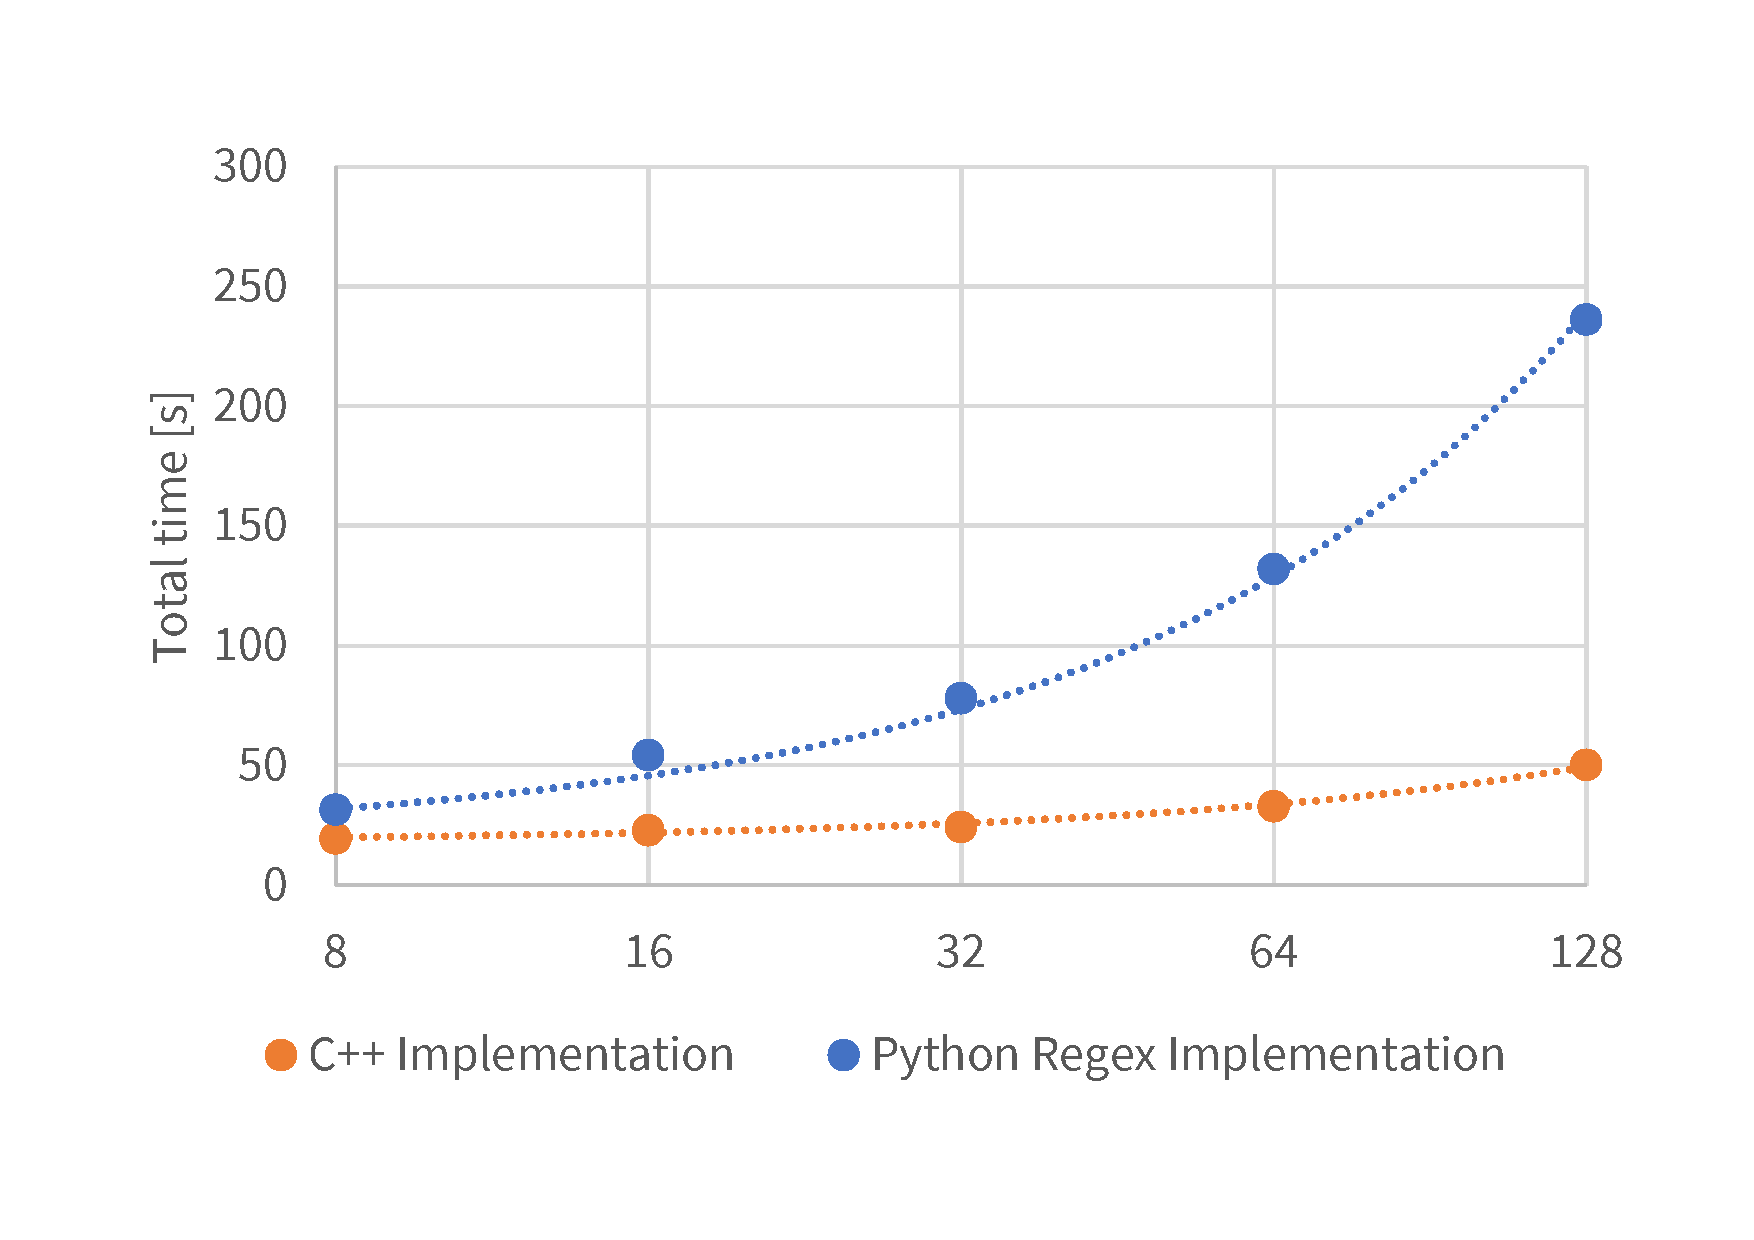
\includegraphics[width=0.8\textwidth]{resource/impl-scaling.pdf}
    \caption{Performance from the new and the old implementation, running with 16 partitions on a local machine and local data.}
    \label{fig:impl-scaling}
\end{figure}

\subsection{Hardware}
Amazon's current generation of EC2 instance types gives the user a choice between 13 different machine types, every one of which is focused on a different type of application
The machines are grouped in five categories, namely 'General Purpose', 'Compute Optimized', 'Memory Optimized', 'Accelerated Computing' and 'Storage Optimized'.
Furthermore, every instance type itself can be of several 'sizes', which mostly indicates the amount of available CPU cores and memory \cite{amazon2017instance}.

For an make an initial selection of which machines are interesting, we argue that machines under the 'Accelerated Computing' category are not relevant as the target application cannot make use of GPUs, and certainly not FPGAs, ruling out the P2, G3 and F1 types. Then, as the amount of persistent storage is hardly an issue, we may rule out the D2 'Dense Storage' instance as well. Next, the X1 instance provides extremely high amounts of RAM, CPU cores and fast SSD storage per instance, but comes at a hefty price. We speculate the application will be unable to utilize all this hardware effectively and therefore rule it out. The T2 instance is meant to provide low baseline performance with relatively limited hardware, but can boost up its clock frequency according to a CPU credit system whenever additional performance is required. Note that this is hardly our use case, but rather something interesting for a web server, so the T2 is also not considered. Finally, as the M3, C3 and R3 instance feature SSD storage at the expense of older hardware with respect to their newer counterparts, we also do not include them.

This leaves us with the general purpose M4, compute optimised C4, memory optimised and R4, and storage optimised I3.
As efficient storage is not deemed a requirement, the I3 might seem like an odd choice, but it also happens to feature very fast networking capabilities (similar to the R4), which makes it interesting anyway.
As an early hypothesis, we expect either the C4 or R4 to be the fastest.
Whichever is faster will give an indication whether computation (C4) or memory (R4) is the dominant factor.
They are likely followed by the I3, whereas the M4 is expected to be slowest.

Test results for a single machine featuring a total of 128 vCPUs (hyperthreads) are shown in \cref{tab:instance-comparison}. Note that these results were obtained using the previously described software optimisations

\begin{table}[H]
	\centering
	\caption{Accumulated completion times of the various steps of the map phase among all vCPUs and the total real application time for relevant instance types @ 16 instances, 8 vCPUs per instance and 2048 total segments}
	\label{tab:instance-comparison}

	\begin{tabular}{lrrrrr}
	\toprule
	Instance	& 	Downl. [s]	& Decompr. [s]	& Parse [s] 	& Total [s]	\\
	\midrule
	% r4.2xlarge	& 163.558	& 415.329		& 295.477	& 180.273 	\\
	% i3.2xlarge	& 175.182	& 410.549		& 292.959	& 186.429	\\
	% m4.2xlarge	& 421.543	& 375.779		& 255.281	& 215.156	\\
	% c4.2xlarge	& 172.387	& 281.658		& 172.199	& 181.939	\\
	r4.2xlarge	&	3038.469	&	7233.797	&	5337.899	&	252.323 \\
	i3.2xlarge	&	2908.101	&	7223.631	&	5322.268	&	261.525 \\
	m4.2xlarge	&	4842.310	&	5687.446	&	3672.714	&	315.539 \\
	c4.2xlarge	&	4112.324	&	5148.951	&	3419.514	&	247.146 \\
	\bottomrule
	\end{tabular}
\end{table}

Observe how the C4, R4 and I3 instances are practically equally fast, with the M4 bringing up the rear as expected.
Moreover, note that the C4 and R4 spend about equal amounts of time on every single stage, implying these machines are very similar to each other.
Indeed, upon having a closer look at their specifications, it appears the I3 is exactly equal to an R4, with added fast SSD storage, making it more expensive (as a spot instance even more so than on-demand).
Furthermore, although the C4 instance is as fast as the R4 and I3, it actually spends more time downloading and significantly less time decompressing and parsing.
Although the latter is to be expected, the fact that it is not faster than the other instances implies a significant networking bottleneck.
The same holds for the M4, but this machine does not have the computational abilities to make up for its lower network bandwidth and is therefore slower.

As a final investigation we look at the amount of vCPUs per instance that delivers the best performance.
One may suspect that higher download speeds can be reached when using multiple small machines, each with a dedicated connection as opposed to using fewer big machines, that share a connection.
As the application is network limited, this would have a profound effect on performance.
\Cref{fig:r4-scaling} gives an indication of how performance scales with the amount of cores per instance.

\begin{figure}[H]
	\centering
	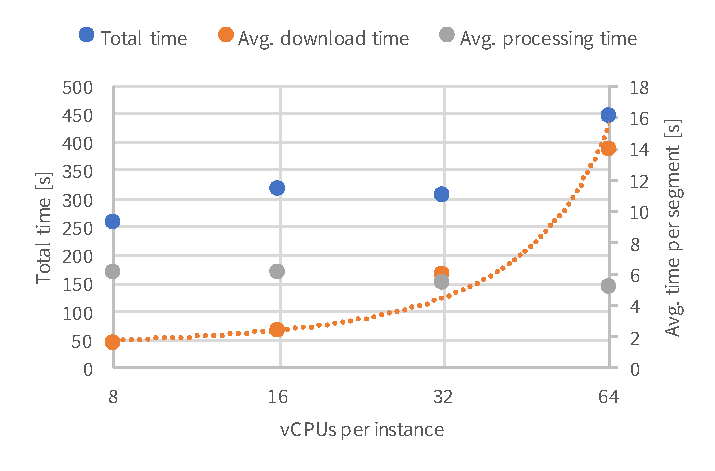
\includegraphics[width=0.8\textwidth]{resource/r4-scaling.pdf}
	\caption{Total real application time and average download and processing times per segment among all cores for R4 models with 8, 16, 32, and 64 vCPUs}
	\label{fig:r4-scaling}
\end{figure}

Note that download times increase linearly with the amount of vCPUs per instance, whereas processing times stay relatively constant.
It can be seen this influences the total execution time significantly, as expected, and that smaller instances are therefore the better choice.
This was further confirmed by inspection of the Ganglia monitor, which showed decreasing network bandwidth usage and suboptimal CPU utilization for clusters of higher amounts of vCPUs.

\section{Results}
As a final measurement we combine the insights from the previous segments to process the entire \num{72000} segment dataset.
The goal will be to process the whole dataset in about an hour.
As the C4, R4 and I3 instances perform equally well, we pick the C4 instance type as it is the cheapest available.
The instance size scaling analysis for the R4 machine from \cref{fig:r4-scaling} is expected to hold for other instance types as well, so the c4.2xlarge with 8 vCPUs is deemed the best choice.

To provide an estimate of the amount of instances that are required to finish within an hour, we calculate the time per segment for a single instance from the results from \cref{tab:instance-comparison}, multiply by the total amount of segments and divide by one hour and round up the result:

\begin{align*}
	\#_{\text{instances, required}} &= \left\lceil\frac{t_{\text{total}} / \#_{\text{segments}} \cdot \#_{\text{instances, used}} \cdot \#_{\text{segments, total}}}{t_{\text{desired}}}\right\rceil \\
	&= \left\lceil\frac{250 / 2048 \cdot 16 \cdot 72000}{3600}\right\rceil \\
	&= 40.
\end{align*}

\section{Conclusion}

\subsection{Recommendations}
More performance can be gained by switching out the \texttt{zlib} decompression library for a faster alternative such as the Intel \texttt{zlib} fork, as a drop-in replacement or for example using \texttt{libdeflate}.
Performance may also be improved by making the module fully streaming compatible, so it can process while it reads or downloads the data in smaller chunks, interleaving the download and computational process.
The streaming part is especially important to lower the memory footprint, but also to mitigate the horrendously slow throughput from S3.
This would eliminate the processing times that are incurred now entirely, because the current implementation is fast enough to never choke on the download speed from S3.
For this lab it was not really seen as appropriate to invest a lot of time into this, for as usual one trades compute time for development time.


\printbibliography
\end{document}
